\documentclass{beamer}
%\usetheme{Ilmenau}
%\usecolortheme{beaver}

\usepackage[slovak,american]{babel}
\usepackage[utf8]{inputenc}
\usepackage{graphicx}
\usepackage{adjustbox}
 \usepackage{xcolor}
 
 \newsavebox\MBox
\newcommand\Cline[2][red]{{\sbox\MBox{$#2$}%
  \rlap{\usebox\MBox}\color{#1}\rule[-2.2\dp\MBox]{\wd\MBox}{1pt}}}

%\usefonttheme{serif}

%\definecolor{UKOrange}{HTML}{ef9424} %
\definecolor{UKOrange}{HTML}{7a2c18} %
\definecolor{UKBrown}{HTML}{a96d5e} %
\definecolor{UKLight}{HTML}{d8b6ab} %
\definecolor{UKDark}{HTML}{7a4f44}
\definecolor{UKDarker}{HTML}{4d312b} 
\definecolor{UKDarkest}{HTML}{2e1e1a}
\definecolor{UKRed}{HTML}{bf1f1c}

\setbeamertemplate{footline}[frame number]{}
\setbeamertemplate{navigation symbols}{}

%\usecolortheme{beaver}
\setbeamertemplate{itemize item}[square]
\setbeamercolor{itemize item}{fg = UKBrown}
\setbeamercolor{itemize subitem}{fg = UKLight}
\setbeamercolor{enumerate item}{fg = UKDark}

\setbeamercolor{footnote}{fg=UKLight}
\setbeamercolor{footnote mark}{fg=UKLight}
\setbeamerfont{footnote}{size=\tiny}
\renewcommand\footnoterule{}

\usetheme{default}
\beamertemplatenavigationsymbolsempty
\setbeamercolor{title}{fg=white, bg=UKBrown}
\setbeamercolor{frametitle}{fg=white, bg=UKBrown}
\setbeamercolor{block title}{bg=UKBrown, fg= white}
\setbeamercolor{block body}{bg =UKLight, fg = UKDarkest}

\setbeamercolor{block title alerted}{bg=UKOrange, fg= white}
\setbeamercolor{block body alerted}{bg =UKLight, fg = UKDarkest}

% odstrani gulicky
\renewcommand*{\slideentry}[6]{}

\useoutertheme[subsection=false]{miniframes}
\AtBeginSection[]{\subsection{}}

\setbeamercolor{below lower separation line head}{bg=UKDark}
\addtobeamertemplate{headline}{}{%
  \begin{beamercolorbox}[colsep=0.5pt]{below lower separation line head}
  \end{beamercolorbox}
}
%\setbeamercolor*{mini frame}{fg=white,bg=UKRosy}
\setbeamercolor{section in head/foot}{fg=UKLight, bg=UKDark}

\usepackage{etoolbox}
\makeatletter
\preto{\@verbatim}{\topsep=0pt \partopsep=0pt }
\makeatother

%\setbeamertemplate{itemize/enumerate body begin}{\normalsize}
%\setbeamertemplate{itemize/enumerate subbody begin}{\normalsize}




%\newcommand{\codeblock}[2]{ \begin{block}{#1} \begin{verbatim}#2\end{verbatim}\end{block}}

%\defbeamertemplate*{title page}{customized}[1][]
%{
%  \begin{centering}
%    \begin{beamercolorbox}[sep=8pt,center]{title}
%      \usebeamerfont{title}\inserttitle
%    \end{beamercolorbox}
%  \end{centering}
%  \bigskip
%
%\begin{columns}[onlytextwidth,T]
%
%
%  \column{27mm}
%  \includegraphics[width=27mm]{images/logoFMFI.png}
%  
%  \column{\dimexpr\linewidth-54mm-6mm}
%  \centering
%  \vspace{5mm}  
%  \usebeamerfont{author}\insertauthor\par
%  \vspace{5mm}
%  \usebeamerfont{institute}\insertinstitute\par
%
%  \column{27mm}
%  \includegraphics[width=27mm]{images/logoUK.png}  
%\end{columns}
%\centering
%\vspace{7mm}
%  \usebeamerfont{date}\insertdate\par
%}



\newcommand{\e}[1]{$\cdot 10^{#1}$}


\title[1. cvičenie]{PSO - základy matlabu}
\author[Kocur]{Ing. Viktor Kocur \\{\small viktor.kocur@fmph.uniba.sk}}
\institute{DAI FMFI UK}
\date{24.9.2020}

\begin{document}
\selectlanguage{slovak}


\begin{frame}

  \titlepage

\end{frame}

\section{Základy matlabu}
\begin{frame}
\frametitle{Prostredie Matlab}

\begin{itemize}
\item Matrix Laboratory of Mathworks
\item Od roku 1984
\item Originálne prostredie na využitie LINPACK-u a EISPACK-u bez znalosti Fortranu
\item Optimalizovaý na mnohé druhy výpočtov - hlavne lin. algebra
\item Jednoduchá implementácia a testovanie algoritmov spracovania obrazu
\end{itemize}
\end{frame}

\subsection{Ako hladať pomoc}

\begin{frame}
\frametitle{Webové zdroje}

Prezentácie a podklady k cvičeniam:
\begin{itemize}
%\item \url{https://www.sccg.sk/~kocur/}
\item \url{https://dai.fmph.uniba.sk/w/Image_Processing_Fundamentals/}
\item \url{https://github.com/kocurvik/edu/}
\end{itemize}


Externé:
\begin{itemize}
\item \url{https://www.mathworks.com/help/matlab/}
\item \url{https://www.mathworks.com/matlabcentral/answers/}
\item \url{https://stackoverflow.com/}
\end{itemize}
\end{frame}

\begin{frame}
\frametitle{Help v Matlabe}
  \begin{block}{Ako nájsť pomoc priamo v Matlabe}
  \begin{itemize}
    \item help command
    \item lookfor keyword
    \item F1
  \end{itemize}
  \end{block}

  \begin{alertblock}{Úloha}
    Otestujte pre príkaz/heslo 'edge'
  \end{alertblock}
  
  \begin{block}{Poznámka}
    V matlabe môžete používať štandardné unixové príkazy ako cd, ls, mkdir, ...
  \end{block}
\end{frame}

\subsection{Premenné a základné operácie}

\begin{frame}[fragile]
\frametitle{Skalárne premenné a aritmetika}

  \begin{block}{Priraďovanie premenných}
  \begin{verbatim}
    a = 1
    a = 1;  \end{verbatim}
  \end{block}
  
  \pause
  
  \begin{alertblock}{Názvy}
    Názvy su case sensitive! Musia začínať písmenom (potom môžu byť aj čísla) a mať max 63 znakov.
  \end{alertblock}
  
  \pause
  
  \begin{block}{Aritmetika}
  \begin{verbatim}
    a = 1 * 2 + 8/9 - 4^(3/2)
    b = a - 1 + 54*24
    a = b*a  \end{verbatim}
  \end{block}
  
  \pause
  
  \begin{alertblock}{Inf a NaN}
  \begin{verbatim}
    1/0 == Inf
    0/0 == NaN  \end{verbatim}
  \end{alertblock}
\end{frame}

\begin{frame}[fragile]
\frametitle{Matematická vsuvka - Maticové násobenie}
  \begin{block}{Definícia}
    $$\mathbb{A} \in \mathbb{R}^{m\times n}, \mathbb{B} \in \mathbb{R}^{n\times l}, \mathbb{C} \in \mathbb{R}^{m\times l}, \mathbb{A} \mathbb{B} = \mathbb{C} \iff$$ \\
    $$\forall i \in \hat{m}, \forall j \in \hat{l}, \mathbb{C}_{i,j} = \sum_{k = 1}^n \mathbb{A}_{i,k} \cdot \mathbb{B}_{k,j}$$
  \end{block}
  
  \begin{alertblock}{Stĺpce vs riadky}
   Značíme $\mathbb{R}^{\textnormal{počet riadkov} \times \textnormal{počet stĺpcov}}$
   a $\mathbb{A}_{\textnormal{riadok}, \textnormal{stĺpec}}$
  \end{alertblock}
  
\end{frame}

\begin{frame}[fragile]
\frametitle{Vektorové premenné}
  \begin{block}{Priraďovanie vektorových premenných}
  \begin{verbatim}
    v = [1 2 3]
    w = [1; 2; 3]  \end{verbatim}
  \end{block}
  
  \pause
  
  \begin{alertblock}{Stĺpcové vs riadkové vektory}
  \begin{verbatim}
    w*v != v*w
    v+w != v+w' \end{verbatim}
  \end{alertblock}
  
  \pause

  \begin{block}{Generovanie vektorov}
  \begin{verbatim}
    r = start:step:end
    r = linspace(start,end,n)  \end{verbatim}
  \end{block}
\end{frame}

\begin{frame}[fragile]
\frametitle{Maticové premenné}
  \begin{block}{Priraďovanie matíc}
  \begin{verbatim}
    A = [1 2 3; 4 5 6]
    B = [v; 2*v - 1]
    C = [w w]  
    D = [A; B]\end{verbatim}
  \end{block}  

\pause

%  \begin{block}{Funkcie na generáciu matíc}
%  \begin{verbatim}
%    zeros(n), zeros(sz), zeros(s1,...,sn)
%    ones(n)
%    eye(n) % Matica identity
%    rand(n) % Náh. matica s rovnomernou dist.
%    randn(n) % Náh. matica s norm. dist.
%    magic(n) % Magická matica  \end{verbatim}
%  \end{block}

  
  \begin{block}{Funkcie na generáciu matíc}
  \begin{itemize}
    \item zeros(n), zeros(sz), zeros(s1,...,sn)
    \item ones(n)
    \item eye(n) - Matica identity
    \item rand(n) - Náh. matica s rovnomernou dist.
    \item randn(n) - Náh. matica s norm. dist.
    \item magic(n) - Magická matica  
    \end{itemize}
  \end{block}  
  \end{frame}
  
\begin{frame}
  \frametitle{Operácie s poliami}
  \noindent\makebox[\textwidth]{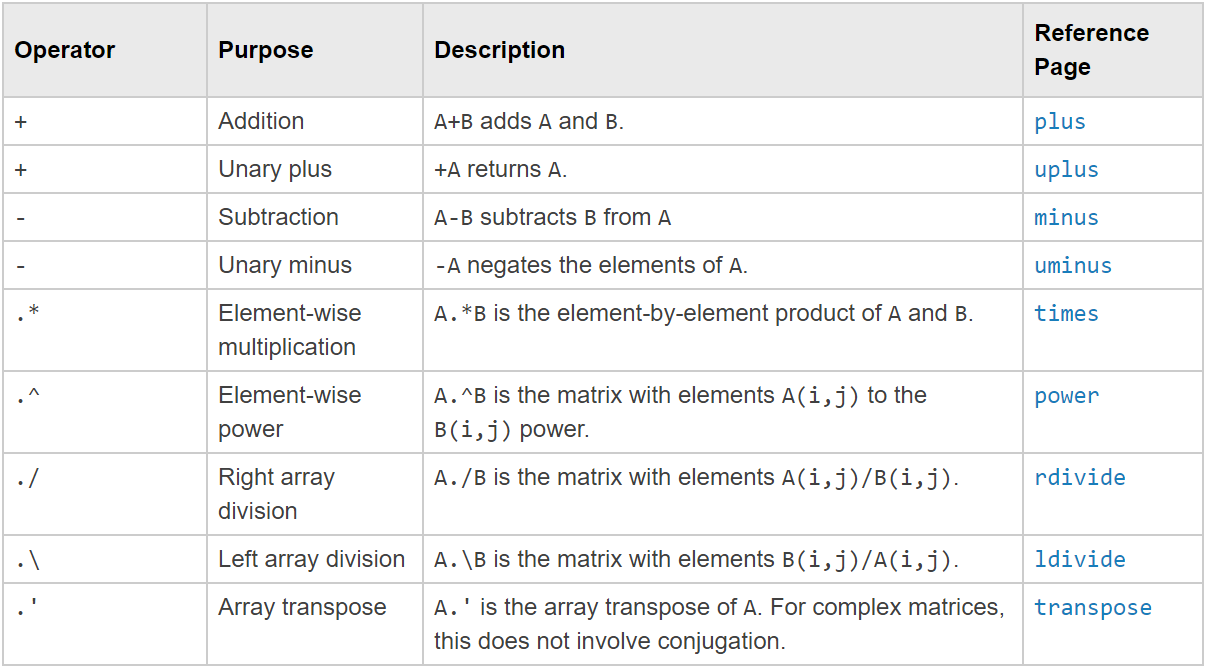
\includegraphics[width=\linewidth]{ArrayOPs.png}}
\end{frame}

\begin{frame}
  \frametitle{Operácie s maticami}
  \noindent\makebox[\textwidth]{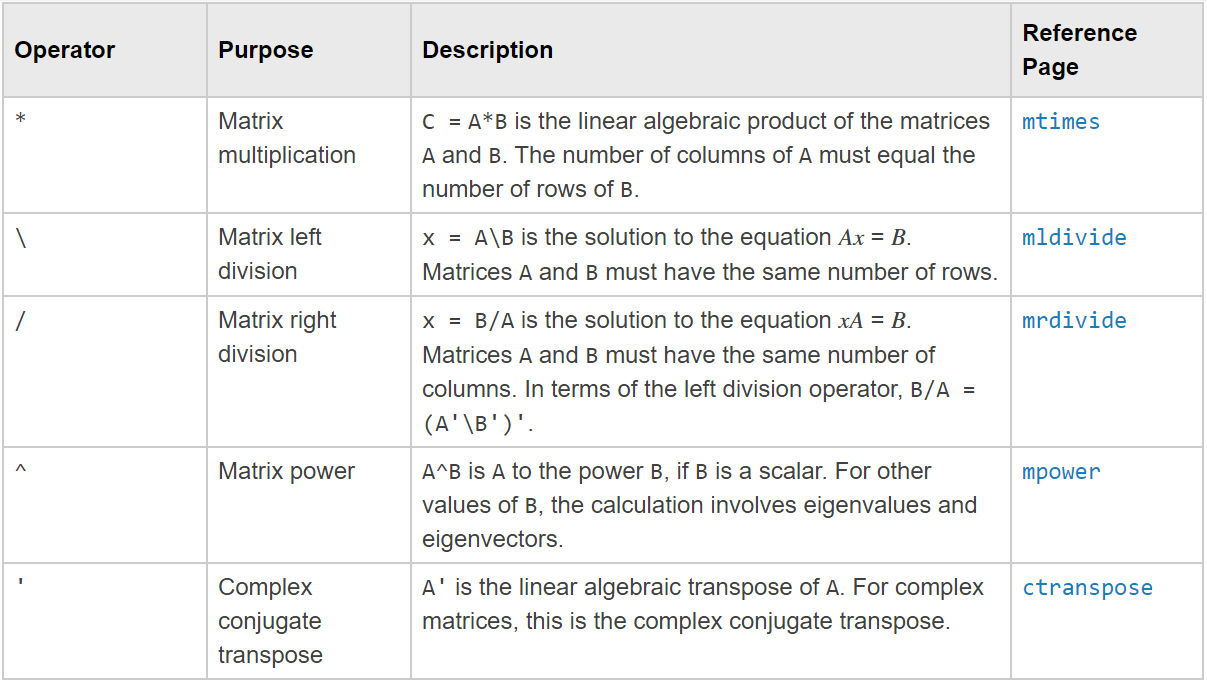
\includegraphics[width=\linewidth]{MatrixOPs.png}}  
  \url{https://www.mathworks.com/help/matlab/matlab_prog/array-vs-matrix-operations.html}
\end{frame}

\begin{frame}[fragile]
  \frametitle{Relačné operácie}
  \begin{block}{Relačné operátory - vracajú typ logical}
  \begin{verbatim}
    <, <=, >, >=, ==, ~=\end{verbatim}  
  \end{block}
  
  \pause
  
  \begin{block}{Porovnávať môžeme aj vektory a matice}
  \begin{verbatim}
    A = rand(5)
    B = rand(5)
    A > B
    A > 0.5 \end{verbatim}
  \end{block}
\end{frame}

\begin{frame}[fragile]
  \frametitle{Logické operácie}
  \begin{block}{Logické funkcie a operátory - vracajú a používajú typ logical}
  \begin{verbatim}
    and (&), or (|), not (~), xor\end{verbatim}  
  \end{block}
  
  \begin{block}{Short-circuit operátory - iba pre skaláry}
  \begin{verbatim}
    &&, ||\end{verbatim}  
  \end{block}
  
  
  \pause
  
  \begin{block}{Redukcia na jednu hodnotu}
  \begin{itemize}
    \item any(a) - Vráti True ak aspoň jeden prvok v a je True
    \item all(a) - Vráti True ak všetky prvky v a sú True
  \end{itemize}
  \end{block}    
\end{frame}


\begin{frame}[fragile]
\frametitle{Funkcie na prácu s maticami}

%  \begin{lstlisting}
%	flip(A)
%	rot90(A)
%	ones(n),ones(s1,...,sn), ones(sz)
%	eye(n), ...
%	zeros(n), ...
%	rand(n)
%	magic(n)
%	transpose(A), A'
%	.OP - prevedie operaciu postupne pre element po elemente
%	repmat(A,n), repmat(A,s1,...,sn)
%	reshape(A,s1,..,sn), reshape(A,sz)
%	size(A)
%  \end{lstlisting}
  
  \begin{block}{Užitočné funkcie}
  \begin{itemize}
    \item flip(A) - Pretočenie matice
    \item rot90(A) - Otočenie matice
    \item transpose(A), A' - Transpozícia matice
    \item inv(A) - Inverzná matica k A
    \item repmat(A,n) - Matica s $n \times n$ podmaticami A 
    \item reshape(A,s1,..,sn) - Zmena tvaru matice
    \item squeeze(A) - Odstránenie 'singleton' dimenzie 
    \item size(A) - Veľkosť matice
    \item numel(A) - Počet prvkov matice    
  \end{itemize}
  \end{block}
  
  Zoznam funkcií na prácu s maticami a poliami: \\
  \url{https://www.mathworks.com/help/matlab/matrices-and-arrays.html}  
\end{frame}

\begin{frame}[fragile]
\frametitle{Úloha na prácu s maticami}
  
  \begin{block}{Zadanie}
  \centering
    Riešte rovnicu $\mathbb{A}\vec{x} = \vec{b}$ \\
    $\mathbb{A} \in \mathbb{R}^{4\times4}, \mathbb{A}_{i,j} = i\cdot (j + 2)$ \\
    $\vec{b} \in \mathbb{R}^4, \vec{b_i} = i^2$
  \end{block}
  
  \pause
  
  \begin{block}{Riešenie napr.}
  \begin{verbatim}
    A = (1:4)'*(3:6)
    b = (1:4).^2
    x = A\b'  \end{verbatim}
  \end{block}  
\end{frame}

\subsection{Indexácia}

\begin{frame}[fragile]
\frametitle{Vektorová indexácia}
  \begin{alertblock}{Pozor}
    Indexy začínajú od 1!
  \end{alertblock}  
    
  \begin{block}{Indexácia}
  \begin{verbatim}
    v = [7 8 5 2 4 6 5 2]
    v(2) == 8
    v(4:6) == [2 4 6]
    v(1:2:end) == [7 5 4 5]
    v([3 6 2]) == [5 6 8]\end{verbatim}
  \end{block}
  
\end{frame}

\begin{frame}[fragile]
\frametitle{Zápis pomocou indexácie}

  \begin{block}{Zápis prostredníctvom indexácie}
  \begin{verbatim}
    v = [7 8 5 2 4 6 5 2]
    v(2) = 4
    v(4:6) = [1 2 3]
    v(1:2:end) = [1 3 5 7]
    v([3 6 2]) = 1
    v(70) = 10000\end{verbatim}
  \end{block}
  
  \pause
  
  \begin{alertblock}{Za koniec vektoru môžeme zapisovať, ale nie číať}
  \begin{verbatim}
    v = [1 2 3]
    v(4) %nebude fungovať
    v(4) = 4 %bude fungovať\end{verbatim}
  \end{alertblock}
\end{frame}

\begin{frame}
\frametitle{Maticová indexácia}
  \begin{alertblock}{Tri spôsoby indexácie}
    Je potrebné rozlišovať medzi troma spôsobmi indexácie matíc!
    \begin{itemize}
      \item jedným indexom
      \item dvojicou (riadok, stĺpec) - obecne n-ticou
      \item logickou maticou
    \end{itemize}
  \end{alertblock}
\end{frame}

\begin{frame}[fragile]
\frametitle{Maticová indexácia - jedným indexom}

  \centering
  
  Pri použití jedného indexu začneme vľavo hore a idem najprv dole po stĺpci, na konci prejdeme na vrch nasledujúceho stĺpca.
    
  $$\begin{bmatrix}
       1 & 4 & 7 & 10 \\[0.3em]
       2 & 5 & 8 & 11 \\[0.3em]
       3 & 6 & 9 & 12 \\[0.3em]
     \end{bmatrix} $$
\end{frame}

\begin{frame}[fragile]
\frametitle{Maticová indexácia - jedným indexom}    
  \begin{block}{Čítanie}
  \begin{verbatim}
    A = magic(5)
    A(4) == 10
    A([4 5 6]) == [10 11 24]
    A([4; 5; 6]) == [10; 11; 24]
    A([10 25; 11 15]) == [18 9; 1 25]
    A(4:4:20) == [10 6 7 8 2]
    A(:) == [17 23 4 10 11 24 5 6 12 ...]\end{verbatim}
  \end{block}
  
\begin{block}{Zápis}
  \begin{verbatim}
    A = magic(5)
    A(4) = 10
    A([4 5 6]) = [10 11 24]
    A([10 25; 11 15]) = [100 200; 300 400]
!!! A([10 25; 11 15]) = [100 200 300 400]\end{verbatim}
  \end{block}
\end{frame}

\begin{frame}[fragile]
\frametitle{Maticová indexácia - dvoma indexmi}    
  \begin{block}{Čítanie}
  \begin{verbatim}
    A = magic(5)
    A(2,2) == 5
    A(:,2) == [24; 5; 6; 12; 18]
    A(1:2:end,1:3)
    A([3 5],3:5)
    A([5 5 4 2 1],[2 4 5])\end{verbatim}
  \end{block}
  
\begin{block}{Zápis}
  \begin{verbatim}
    A = magic(5)
    A(2,2) = 1000
    A(1:2:5,1:end-2) = eye(3)
!!! A(1:2:5,1:3) = [1 2 3 4 5 6 7 8 9]
!!! A([5 5],1) = [1 2]\end{verbatim}
  \end{block}   
\end{frame}

\begin{frame}[fragile]
\frametitle{Maticová indexácia - logickou maticou}    
  \begin{block}{Čítanie a zápis}
  \begin{verbatim}
    A = rand(5)
    L = A>0.5    
    A(L)
    A(L) = 0 
    B = magic(5)
    B(A < 0.3 | L) = 50 \end{verbatim}
  \end{block}
  
  \pause
  
  \begin{alertblock}{Pozor na rozmery}
    Logická matica musí mať rovnaký rozmer ako matica s ktorou operujeme
  \end{alertblock}   
\end{frame}

\begin{frame}[fragile]
\frametitle{Maticová indexácia - prechody}    
  \begin{block}{Funkcie na prechod}
  \begin{verbatim}
    [r,c] = ind2sub(sz,idx)
     idx  = sub2ind(sz,r,c)
     idx  = find(logicalMatrix)\end{verbatim}
  \end{block}  
  
  \pause
  
\begin{block}{Zápis do prázdneho indexu mimo matice}
  \begin{verbatim}
    A = magic(5)
!!! A(26) = 1  % nefunguje - nejednoznačné
    A(6,1) = 1 % funguje \end{verbatim}
  \end{block}   
\end{frame}

\begin{frame}[fragile]
\frametitle{Úloha na indexáciu 1}
 
  \begin{block}{Zadanie}
    Vygenerujte maticu pomocou rand(8). Premente všetky prvky ktoré by boli na šachovnici na čiernom políčku na 1. Následne premente všetky prvky menšie ako 0.3 na 0. 
  \end{block}
  
  \noindent\makebox[\textwidth]{
\includegraphics[width=0.2\linewidth]{chessboard.jpg}}  
  
  \pause
  
  \begin{block}{Riešenie napr:}
  \begin{verbatim}
    R = rand(8)
    R(1:2:7,2:2:8) = 1
    R(2:2:8,1:2:7) = 1
    R(R<0.3) = 0 \end{verbatim}
  \end{block}  
\end{frame}

\begin{frame}[fragile]
\frametitle{Úloha na indexáciu 2}
 
  \begin{block}{Zadanie}
    Vygenerujte maticu pomocou magic(8) a z nej vytvorte maticu 8x4 len z prvkov na bielych políčkach.
  \end{block}
  
  \noindent\makebox[\textwidth]{
\includegraphics[width=0.2\linewidth]{chessboard.jpg}}  
  
  \pause
  
  \begin{block}{Riešenie napr:}
  \begin{verbatim}
    A = magic(8)
    s = [1 0;0 1]
    I = repmat(s,4)
    B = reshape(A(I == 1),[8 4]) \end{verbatim}
  \end{block}  
\end{frame}

\begin{frame}
\frametitle{Matematické funkcie}
 
  \begin{block}{Príklady funkcií}
    \begin{itemize}
      \item mod, round, floor, ceil
      \item abs, sgn, exp, log, sin, cos, tan, asin...
      \item min, max
      \item sum, diff, mean, var
    \end{itemize}
  \end{block}
 
  Viac na \url{https://www.mathworks.com/help/matlab/functionlist.html}
  
  \begin{alertblock}{Treba čítať dokumentáciu}
    Napríklad príkaz sum aplikovaný na maticu vráti riadkový vektor so súčtami hodnôt v jednotlivých stĺpcoch. Ak chceme sčítať všetky prvky matice musíme použiť sum(sum(A)), alebo sum(A(:)). Toto platí aj pre min, max, mean, var, diff...
  \end{alertblock}  
\end{frame}

\subsection{Dátové typy}

\begin{frame}[fragile]
\frametitle{Dátové typy}
 
  \begin{block}{Numerické typy}
    \begin{itemize}
      \item single, double
      \item int8, int16, int32, int64
      \item uint8, uint16, uint32, uint64
    \end{itemize}
  \end{block}
  
  \pause
  
  \begin{block}{Ostatné typy}
  \begin{itemize}
      \item char, string
      \item cell array, map, table, categorical array, struct, logical
      \item date, time, time series, timetable
      \item function handle, handle
  \end{itemize}
  \end{block}
  
  \pause
  
  \begin{block}{Zistenie typu}
  \begin{verbatim}
    class(a)
    whos a \end{verbatim}
  \end{block}
\end{frame}
  
\begin{frame}[fragile]
\frametitle{Numerické typy}   
  
  \begin{block}{Zmena typov}
    \begin{verbatim}
    a = 150
    class(a) == 'double'
    b = uint16(a)
    class(b) == 'uint16'
    cast(int8(-50),'uint8') == 0
    typecast(int8(-50),'uint8') == 206
    typecast(-50,'int16') == [0 0 0 0 0 0 73 192]\end{verbatim}    
  \end{block}  
  
  \pause
  
  \begin{alertblock}{Integer overflow}
    \begin{verbatim}
    uint8(200) + uint8(200) == 255 \end{verbatim}
  \end{alertblock}
  
  \pause
  
  \begin{block}{Zmena vypisovania čísel}
    \begin{verbatim}
    format long
    format shortEng
\end{verbatim}    
  \end{block}  
\end{frame}

\begin{frame}[fragile]
\frametitle{Krátko k niektorým iným typom}   
  
  \begin{block}{Cell array}
    \begin{verbatim}
    c = {45, ones(5), 'hello', [1 2 3]}
    c(1) == {[45]}
    c{1} == 45
    c{3} = 5.24754 \end{verbatim}    
  \end{block}  
  
  \pause
  
  \begin{block}{Struct}
    \begin{verbatim}
    s.a = 1;
    s.b = {'A','B','C'}
    s = 
     struct with fields:
      a: 1
      b: {'A'  'B'  'C'}
    p = struct('fieldName',fieldVal) \end{verbatim}
  \end{block}  
\end{frame}

\section{Skripty a funkcie}

\subsection{Skripty}

\begin{frame}
\frametitle{Skripty}
  \begin{block}{Skripty}
    Skripty ukladáme do samostatného súboru s príponou .m 
  \end{block}
  
  \begin{block}{Spúštanie}
  \begin{itemize}
      \item Spúštanie z command window - príkaz je totožný s názvom súboru (musíme byť v správnej zložke, resp. mať zložku v PATH)
      \item Spúštanie z editoru - možnosť debugovania
  \end{itemize}
  \end{block}
  
  \pause
  
  \begin{alertblock}{Pozor!}
    Skript má prístup k premenným z workspace!
  \end{alertblock}  
\end{frame}
    
\subsection{Funkcie}

\begin{frame}
\frametitle{Funkcie}
  \begin{block}{Funkcie}
    Funkcie ukladáme obdobne ako skripty do samostatného súboru s príponou .m. Na rozdiel od skriptov maju funkcie vstupy a výstupy.
  \end{block}
  
  \pause
  
  \begin{block}{Spúštanie}
    Funkciu voláme príkazom podľa názvu SÚBORU. Súbor musí byť uložený v pracovnej zložke, alebo zložke ktorá je v Matlabovskom PATH. 
  \end{block}
  
\end{frame}

\begin{frame}[fragile]
\frametitle{Funkcie - štruktúra}
  \begin{block}{Funkcie}
  \begin{verbatim}
    function output = functionName(input)
    % comment - bude sa zobrazovat v helpe
        output = 2*input;
    % tento comment sa uz nezobrazi v helpe
    end \end{verbatim}
  \end{block}
  
\end{frame}

\begin{frame}[fragile]
\frametitle{Funkcie - štruktúra}
  
  \begin{block}{Viac vstupov a výstupov}
  \begin{verbatim}
    function [out1,out2] = functionName(in1,in2)
        out1 = 2*in1;
        out2 = in1*in2;
    end \end{verbatim}
  \end{block}

  \begin{block}{Variabilný počet vstupov a výstupov}
    Pre variabilný počet vstupov môžeme použiť špeciálne premenné nargin (počet vstupov) a varargin (pole vstupov variabilnej dĺžky) pre vstupy a nargout pre výstupy.
  \end{block}
\end{frame}

\begin{frame}[fragile]
\frametitle{Funkcie - nested a local}
  \begin{block}{Funkcie}
  \begin{verbatim}
    function parent
        disp('This is the parent function')
        nestedfx
        localfx

        function nestedfx
            disp('This is the nested function')
        end
    end 
    
    function localfx
        disp('This is a local function')
    end\end{verbatim}
  \end{block}
\end{frame}

\begin{frame}
\frametitle{Funkcie}
  \begin{block}{Nested Funkcie}
    Majú prístup k premenným parent funkcie a naopak. Ak však použijú premennú, ktorá nieje definovaná v parent funkcii, tak táto hodnota sa stratí po konci volania nested funkcie.
  \end{block} 

  \begin{block}{Local funkcie}
    Nemajú prístup k premenným parent funkcie.
  \end{block}  
\end{frame}

\begin{frame}[fragile]
\frametitle{Anonymné funkcie}
  \begin{block}{Príklad}
  \begin{verbatim}
    sqr = @(x) x.^2;
    sqr(5) == 25
    
    q = integral(sqr,0,1);
    q = integral(@(x) x.^2,0,1); \end{verbatim}
  \end{block}
\end{frame}

\subsection{Control Flow}

\begin{frame}[fragile]
\frametitle{If}
  \begin{block}{Štruktúra}
  \begin{verbatim}
    if expression
        statements
    elseif expression
        statements
    else
        statements
    end \end{verbatim}
  \end{block}
\end{frame}

\begin{frame}[fragile]
\frametitle{Switch}
  \begin{block}{Štruktúra}
  \begin{verbatim}
    switch switch_expression
        case case_expression
            statements
        case case_expression
            statements
            ...
        otherwise
            statements
    end \end{verbatim}
  \end{block}
\end{frame}

\begin{frame}[fragile]
\frametitle{For cyklus}
  \begin{block}{Štruktúra}
  \begin{verbatim}
   for index = values
       statements
   end
   
   for i = 1:n
       	r(i) = ...
   end
   
   for i = [5 0 2 7 5 1]
       	statements
   end \end{verbatim}
  \end{block}
\end{frame}

\begin{frame}[fragile]
\frametitle{While cyklus}
  \begin{block}{Štruktúra}
  \begin{verbatim}
    while expression
       statements
    end \end{verbatim}
  \end{block}
  
  \pause
  
  \begin{block}{Predčasné ukončenie while a for cyklu}
  \begin{itemize}
      \item break - ukončí celý cyklus
      \item continue - prejde na ďalšiu iteráciu cyklu
  \end{itemize}
  \end{block}
  
  \pause
  
  \begin{alertblock}{Terminácia programu}
    Akýkoľvek skript a funkciu môžeme ukončiť stlačením Ctrl-C
  \end{alertblock}  
\end{frame}

\begin{frame}
\frametitle{Úloha}
  \begin{block}{Zadanie}
  Napíšte funkciu fib(n), ktorá vráti n-tý člen Fibonacciho postupnosťi.
  \end{block}

  \begin{block}{Zadanie - ťažká verzia}
  Napíšte funkciu na lineárne rekurentnú postupnosť linrek(n,$\vec{a}$,$\vec{b}$), ktorá vráti n-tý člen lineárnej rekurentnej postupnosti v tvare $$f_n = \sum_{i = 1}^{dim(\vec{a})} a_i \cdot f_{n-i},$$ s počiatočnými hodnotami $f_i = b_i$ pre $i \leq dim(\vec{a}) = dim(\vec{b})$.
  \end{block}
\end{frame}  

\begin{frame}[fragile]
\frametitle{Úloha - riešenie}
    \begin{block}{Riešenie napr.:}
  \begin{verbatim}
    function out = fib(n)
        if n <= 0
            out = 0;
        elseif n == 1
            out = 1;
        else
            out = fib(n-1) + fib(n-2)
        end
    end \end{verbatim}
  \end{block}
  \pause  
  \begin{block}{Alebo:}
  \begin{verbatim}
    function out = fib(n)
        out = round(1.61803398875^(n-1))
    end \end{verbatim}
  \end{block}
\end{frame}  

\begin{frame}[fragile]
    \begin{block}{Riešenie ťažšej verzie napr:}
  \begin{verbatim}
    function rek = linrek(n,a,b)
        if length(b) >= n
            rek = b(n);
        else
            rek = 0;
            for i=1:length(b)
                rek = rek + a(i) * linrek(n-i,a,b);
            end
        end
    end \end{verbatim}
  \end{block}
\end{frame}

\begin{frame}[fragile]
\frametitle{Úloha - bez rekurzie}
  \begin{block}{Riešenie napr:}
  \begin{verbatim}
    function rek = linrekaprox(n,a,b)
        pol = [-1 a];
        r = roots(pol)';
        m = zeros(size(r));
        for i = 1:numel(a)
            m(i) = sum(r(1:i) == r(i)) - 1;
        end
        rowmat = repmat((1:numel(a))',1,numel(a));
        A = (r.^rowmat).*(rowmat.^m);
        k = A\b';
        rek = round(real(((n.^m).*(r.^n))*k));
    end \end{verbatim}
  \end{block}
\end{frame}

\subsection{Meranie doby behu}

\begin{frame}[fragile]
\frametitle{Meranie doby behu}
  \begin{block}{Tic Toc}
  \begin{verbatim}
    tic
    statements
    toc \end{verbatim}
  \end{block}
  
  \begin{block}{Cputime}
  \begin{verbatim}
    t1= cputime
    statements
    t2 = cputime
    disp(t2 - t1) \end{verbatim}
  \end{block}
\end{frame}

\begin{frame}[fragile]
\frametitle{Optimalizácia matlabu - porovnajte doby behov}
  \begin{block}{Bez alokácie}
  \begin{verbatim}
    p = 0;
    for k=1:10000
        p(k) = k/(sin(k)+2)
    end \end{verbatim}
  \end{block}
  
  \begin{block}{S alokáciou}
  \begin{verbatim}
    p = zeros(1,10000)
    for k=1:10000
        p(k) = k/(sin(k)+2)
    end \end{verbatim}
  \end{block}
  
  \begin{block}{Vektorovo}
  \begin{verbatim}
    k = 1:10000
    p = k./(sin(k)+2) \end{verbatim}
  \end{block}
\end{frame}

\section{Práca s obrázkami}

\subsection{Kreslenie grafov}

\begin{frame}[fragile]
\frametitle{Plot}
  \begin{block}{Jednoduchý plot}
  \begin{verbatim}
    x = linspace(0,10,1000);
    plot(x,sin(x)) \end{verbatim}
  \end{block}
  
  \begin{block}{Viac argumentov}
  \begin{verbatim}
    plot(X,Y,LineSpec) 
    plot(X1,Y1,...,Xn,Yn)
    plot(____, Name, Value) \end{verbatim}
  \end{block}
  
   \begin{block}{Linespec - príklady}
   \begin{itemize}
    \item Linestyle - -, --, :, -.
    \item Marker - o, +, *, ., x, s, d
    \item Farby - y, m, c, r, g, b, w, k $\rightarrow$ kombinujeme napr. r*-
   \end{itemize}
  \end{block}
\end{frame}

\begin{frame}[fragile]
\frametitle{Práca s obrázkami}
  \begin{block}{Hold on a hold off}
  \begin{verbatim}
    x = linspace(0,10,1000);    
    plot(x,sin(x))
    hold on
    plot(x,cos(x)) % druhy plot sa nakresli do prveho
    hold off 
    plot(x,cos(x)) % tento plot prekresli prve dva \end{verbatim}
  \end{block}
  
  \pause
  
  \begin{block}{Figure a Axes}
  \begin{verbatim}
    fig1 = figure % vytvori okno
    ax1 = axes % vytvori kartezsky podklad  \end{verbatim}
  \end{block}
  
  \pause
  
  \begin{block}{Kam sa kreslia grafy}
    Grafy sa kreslia do aktívnej figure (gcf) a aktívnych axes (gca). Ak chceme kresliť inam použijeme napr. plot(\_\_\_\_,'Parent',ax4)
  \end{block}
\end{frame}

\begin{frame}[fragile]
\frametitle{Subplot}
  \begin{block}{Viac plotov v jednej figure}
  \begin{verbatim}
    ax1 = subplot(2,2,1);
    plot(x,sin(x))       
    ax2 = subplot(2,2,2);
    plot(x,cos(x))
    ax3 = subplot(2,2,3);
    ax4 = subplot(2,2,4);
    plot(x,x.^2,'Parent',ax3)
    plot(x,x.^3,'Parent',ax4) \end{verbatim}
  \end{block}
\end{frame}

\begin{frame}
\frametitle{Ine grafy a mazanie}
  
   \begin{block}{Ostatné druhy grafov}
   \begin{itemize}
    \item plot3, loglog, semilogx, semilogy, errorbar
    \item bar, bar3, barh, barh3, histogram, pie, pie3
    \item stem, stairs, scatter
    \item countour, countourf, surf, ezsurf
    \item feather, quiver, compass
   \end{itemize}
  \end{block}
  
  \pause 
  
   \begin{block}{Mazanie}
   \begin{itemize}
    \item cla, clf - mažú aktívne axis/figure
    \item close all - zavri všetky figure okná
   \end{itemize}
  \end{block}
\end{frame}

\subsection{Práca s obrázkami}

\begin{frame}[fragile]
\frametitle{Načítanie obrázkov}
  
  \begin{block}{Obrázky}
    Stiahnite si zip z githubu kocurvik/edu/PSO/supplementary
  \end{block}
  
  \pause 
  
  \begin{block}{Načítanie súborov}
  \begin{verbatim}
  rgb = imread('zatisie.jpg');
  whos rgb
  d = im2double(rgb)
  whos d
  bw = imread('zatisie.pgm');
  whos bw \end{verbatim}  
  \end{block}
\end{frame}

\begin{frame}[fragile]
\frametitle{Zobrazovanie} 
  \begin{block}{Zobrazovanie pomocou imshow}
  \begin{verbatim}
     imshow(rgb)
     imshow(d)
     imshow(bw)   \end{verbatim}  
  \end{block}
  
  \pause
  
  \begin{block}{Zobrazovanie pomocou image}
  \begin{verbatim}
     image(rgb)
     image(d)
     imagesc(bw)
     colormap(gray)   \end{verbatim}  
  \end{block}
\end{frame}

\begin{frame}[fragile]
\frametitle{Zápis} 
  \begin{block}{Zápis pomocou imwrite}
  \begin{verbatim}
     imwrite(rgb, 'filename.png')
     imwrite(d, 'filename.jpg')
     imwrite(bw, 'filename.png')   \end{verbatim}  
  \end{block}
  
  \begin{alertblock}{Pozor!}
  Ak je obrázok v uint8, tak očakávaný rozsah je 0-255. Ak je obrázok v double, tak očakávaný rozsah je 0-1. Väčšinou, čo ukáže imshow to zapíše imread. O image a hlavne imagesc to obecne neplatí! 
  \end{alertblock}
\end{frame}

\begin{frame}[fragile]
\frametitle{Úloha} 
  \begin{block}{Zrušenie farebnej zložky}
    Vo farebnom obrázku zátišia znížte červenú zložku RGB na pätinu. Hint: pole je tvaru riadky x stĺpce x farba.
  \end{block}
  
  \pause
  
  \begin{block}{Riešenie}
  \begin{verbatim}
    rgb(:,:,1) = 0.2 * rgb(:,:,1); 
    imshow(rgb)   \end{verbatim}  
  \end{block}
\end{frame}

\begin{frame}[fragile]
\frametitle{Úloha} 
  \begin{block}{Scale}
    Vytvorte funkciu myimresize(I,s), ktorá vráti obrázok zväčšený pomerom s pomocou metódy nearest point interpolation. Porovnajte s funkciu imresize.
  \end{block}
  
  \pause
  
  \begin{block}{Riešenie}
  \begin{verbatim}
function I = myimresize(I, s)
    oldrows = size(I,1);
    oldcols = size(I,2);
    r = round(linspace(1,oldrows,round(s*oldrows)));
    c = round(linspace(1,oldcols,round(s*oldcols)));
    I = I(r,c);        
end  \end{verbatim}  
  \end{block}
\end{frame}

\end{document}